\chapter{Experiments}
In this chapter, previously mentioned methods in chapter \textbf{\ref{Method}} were examined both on a lab-computer and the on-board hardware in real-time. This chapter is conducted under three main topics. First, the experimental procedure will be explained in terms of%todo 
. Second, evaluation of localization algorithm will be done by two different data-sets which are called MIA and KITTI sets are explained in detail in section \textbf{\ref{MIA-set}} and \textbf{\ref{KITTI-set}} respectively. Finally, results of the experiments will be presented and all remarks will be listed as well.

\section{Experimental Procedure}
To cover different aspects of real-world conditions, experiments should be designed in a wide spectrum. Therefore, we conducted several experiments in a different environment and different weather conditions as much as possible by using two different data set for evaluation of the localization algorithms. Experiments were performed in two ways. However, before making experiments, there are some preliminary works need to be done which are described in following section. %todo explain in more detail
\subsection{Preliminary Work}
\subsection*{Sensor Positioning} 
First work was determining position of sensors, which are especially velodyne and imu, w.r.t the center of the car. This part is crucial because it is a backbone for building an accurate map and perform localization algorithm properly. \\
\subsection*{Building Map}\label{mapping}
Second work was building a map of the surrounding where was the test area for experiments. For this purpose, the car was driven around in a test area in order to collect related sensory data e.g. point clouds for creating a three-dimensional map as shown in Figure \ref{fig:bassum}. This work needs to have quite much time for building map. Due to the course of this thesis, this part was not truly examined but it needs roughly one whole day to create the map of 250m radii area.

\begin{figure}[h!]
    \centering
    \includegraphics[scale=0.225]{bassum}
    \captionsetup{singlelinecheck=false}
    \caption{Bassum 3D map}%todo add comment
    \label{fig:bassum}
\end{figure}

\subsection*{Down Sampling}
Final work was applying filter on map data and raw velodyne data. The aim of this work decrease computational time and complexity of both map and velodyne data.
\\
\begin{figure}[h!]
    \begin{subfigure}{.5\textheight}
        \includegraphics[scale=0.3]{no_filter.png}
        \caption{\textbf{Original Map:} It comprises 71,120,230 points and its size is 1.00 GB }
        \label{fig:no_filter}
    \end{subfigure}
    \begin{subfigure}{.5\textheight}
        \includegraphics[scale=0.3]{filtered_rh.png}
        \caption{\textbf{Down-sampled Map:}It contains 1,284,489 points voxel size 3 m its size is 100MB}
        \label{fig:filter_rh}
    \end{subfigure}
    \label{fig:filter}
    \caption{3D map comparison}
\end{figure}
\\
\\
As seen in Figure \ref{fig:no_filter}, the map contains a large amount of redundant information i.e. the surface of objects in the map are represented by a set of points that are more than needed points to depict the surface of the object. Therefore, the original map needs to be down-sampled as shown in Figure \ref{fig:filter_rh}. For down-sampling, it was used an algorithm that is provided by Ros package is Voxel-filer%comment:The VoxelGrid class creates a 3D voxel grid (think about a voxel grid as a set of tiny 3D boxes in space) over the input point cloud data. Then, in each voxel (i.e., 3D box), all the points present will be approximated (i.e., downsampled) with their centroid. This approach is a bit slower than approximating them with the center of the voxel, but it represents the underlying surface more accurately.
. The concept of this filter finding the centroid of points $(C_{x}, C_{y})$ within voxel cell is shown in Figure \ref{fig:voxel} as described following equations:
\begin{equation}
C_{x} =\dfrac{1}{6A}\sum_{i=0}^{n-1}(x_{i}+x_{i+1})(x_{i}y_{i+1}-x_{i+1}y_{i})
\end{equation}
\begin{equation}
C_{y} =\dfrac{1}{6A}\sum_{i=0}^{n-1}(y_{i}+y_{i+1})(x_{i}y_{i+1}-x_{i+1}y_{i})
\end{equation}\\
and where A is the polygon's signed area,\cite{centroid} as described by
\begin{equation}
A =\dfrac{1}{2}\sum_{i=0}^{n-1}(x_{i}y_{i+1}-x_{i+1}y_{i})
\end{equation}

\begin{figure}[h]
\centering
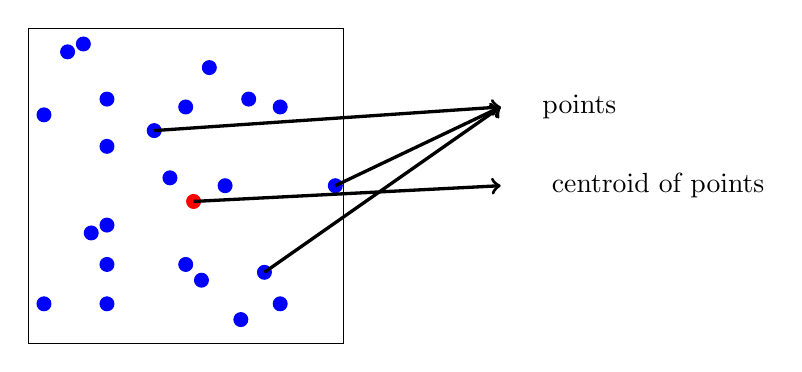
\begin{tikzpicture}
\draw (0,0) -- (4,0) -- (4,4) -- (0,4) -- (0,0);
\draw [blue] plot [only marks, mark size=2.5, mark=*] coordinates {(0.2,0.5) (1,1.5) (1,2.5) (2,1) (3.9,2) (1,1) (2,3) (2.5,2) (1,0.5) (2.3,3.5) (2.8,3.1)
(1.8,2.1) (0.8,1.4) (3.2,3) (1.6,2.7) (2.2,0.8) (2.7,0.3) (3,0.9) (3.2,0.5) 
(0.5,3.7) (1,3.1) (0.2,2.9) (0.7,3.8)};
\draw [red] plot [only marks, mark size=2.5, mark=*] coordinates {(2.1,1.8)};
 \draw [->,very thick](1.6,2.7) -- (6,3) ;
 \draw [->,very thick](3.9,2) -- (6,3) ;
 \draw [->,very thick](3,0.9) -- (6,3) ;
 \draw [->,very thick](2.1,1.8) -- (6,2) ;
 \node[align=left] at (7,3) {points};
 \node[align=left] at (8,2) {centroid of points};
\end{tikzpicture}
 \caption{Voxel cell }
 \label{fig:voxel}
\end{figure}
\subsection{MIA Data Set}\label{MIA-set}
To make data set, MIA car which is equipped several sensors such as velodyne (lidar), imu, radar, cameras etc. was driven in three different vicinity in Bremen. The first place was Jeddeloh where is closed to traffic. The circumference of this area is approximately 785 m and road condition is gravel. Even though the road is gravel, it is relatively even in respect to height. As a note, this condition of the road does not have a big impact on scan registration unlike odometry calculation. The affect of the road condition was discussed in section \ref{sec:discussion}
\\ 
\par The second place was Bassum where is also closed to traffic and separated into two part. First part is relatively empty and homogeneous comparing to the second part where is a track for go-kart as shown in Figure \ref{fig:bassum}. The length of the track is 780 m and the road is asphalt.
\\ 
\par Final place was Robert Hook Strasse and it's around where is open to traffic. In the last place, the environment is dynamically changing, in particular,  positions of a car, pedestrian, cyclist etc. In contrast to that, everything was static in the first two places.  
\\ 
\par These data sets consist of laser point clouds, gps, wheel position, acceleration and angular rotation in respect of x, y, z and roll, yaw, pitch respectively.

\subsection{KITTI Data Set}\label{KITTI-set}
To compare and evaluate our data and localization algorithms, KITTI data set, which is provided  Karlsruhe Institute of Technology
and Toyota Technological Institute, was used. Even though the KITTI of interest is visual odometry, optical flow and etc., provided data set is showing similarity with our data set, in sense of used sensors. Hence, the KITTI data set was utilized for comparing the outputs of the localization methods with KITTI ground truth.
\newpage
\section{Result}\label{sec:result}